\documentclass{report}

\usepackage[utf8]{inputenc}
\usepackage{graphicx}
\usepackage{glossaries}

\begin{titlepage}
   \begin{center}
       \vspace*{1cm}

       \textbf{Thesis Title}

       \vspace{0.5cm}
        Thesis Subtitle
            
       \vspace{1.5cm}

       \textbf{Author Name}

       \vfill
            
       A thesis presented for the degree of\\
       Doctor of Philosophy
            
       \vspace{0.8cm}
     
       \includegraphics[width=0.4\textwidth]{university}
            
       Department Name\\
       University Name\\
       Country\\
       Date
            
   \end{center}
\end{titlepage}
\begin{document}

\tableofcontents{}

\clearpage

\chapter{Introduction}

This project was created as part of the mobile development course led by Mr. Philipe Esling. Autotweet is a Twitter monitoring and automation system. It is composed of a React Native client and an intermediary server.

\section{Project Management}
Three students participated in this project as individual contributors. Mathieu Pionnier is an apprentice at Rami, Thomas Chastaingt at CCI and Aymerick Valette at PayFit. 

The three contributors worked together in a variety of collaboration formats depending on the context. Initially, we tried a workflow consisting of changelists followed by reviews. We quickly realised that it was hard to have a consensus about the project’s base architecture. Changelists were going all over the place without a proper vision. We concluded that it was too early to allow for asynchronous collaboration. We started doing pair-programming sessions to allow for more efficient progression. As a result, we have been able to move faster and communicate better. This workflow also allowed us to review previous changes faster. In parallel to this workflow, the development of the server component was operated solely by Aymerick Valette.

\clearpage

\chapter{Product}

As the bachelor's degree is business-oriented, we wanted to approach the problem as if it were a company project. So, we started the project by first thinking about the product aspect. We tried to create an attractive and useful product while respecting the instructions of the exercise. In hindsight, this was a good decision because we enjoyed working on the project. However, we lost time working on components that were not requested. The project is partially completed because of this.

\section{Features}
Autotweet allows a Twitter user to:
\begin{itemize}
\item Login using its account
\item Get indicators about its Twitter popularity
\item See a graph that represents its popularity over time
\item See a leaderboard that contains its most active followers
\item Send tweets automatically over a time range
\item Answer to tweets automatically

\end{itemize}

\section{User Interface}
Rather than describing the product on paper, here are the GUI prototypes in the figure \ref{fig:gui} and \ref{fig:gui2}. We have created a conventional user interface that is meant to "look" native. The design principles are taken from the Google's Material Design, and from the Apple's HIG guidelines. We first used Sketch and then Figma to collaborate in real-time.

\begin{figure}[htp]
    \centering
    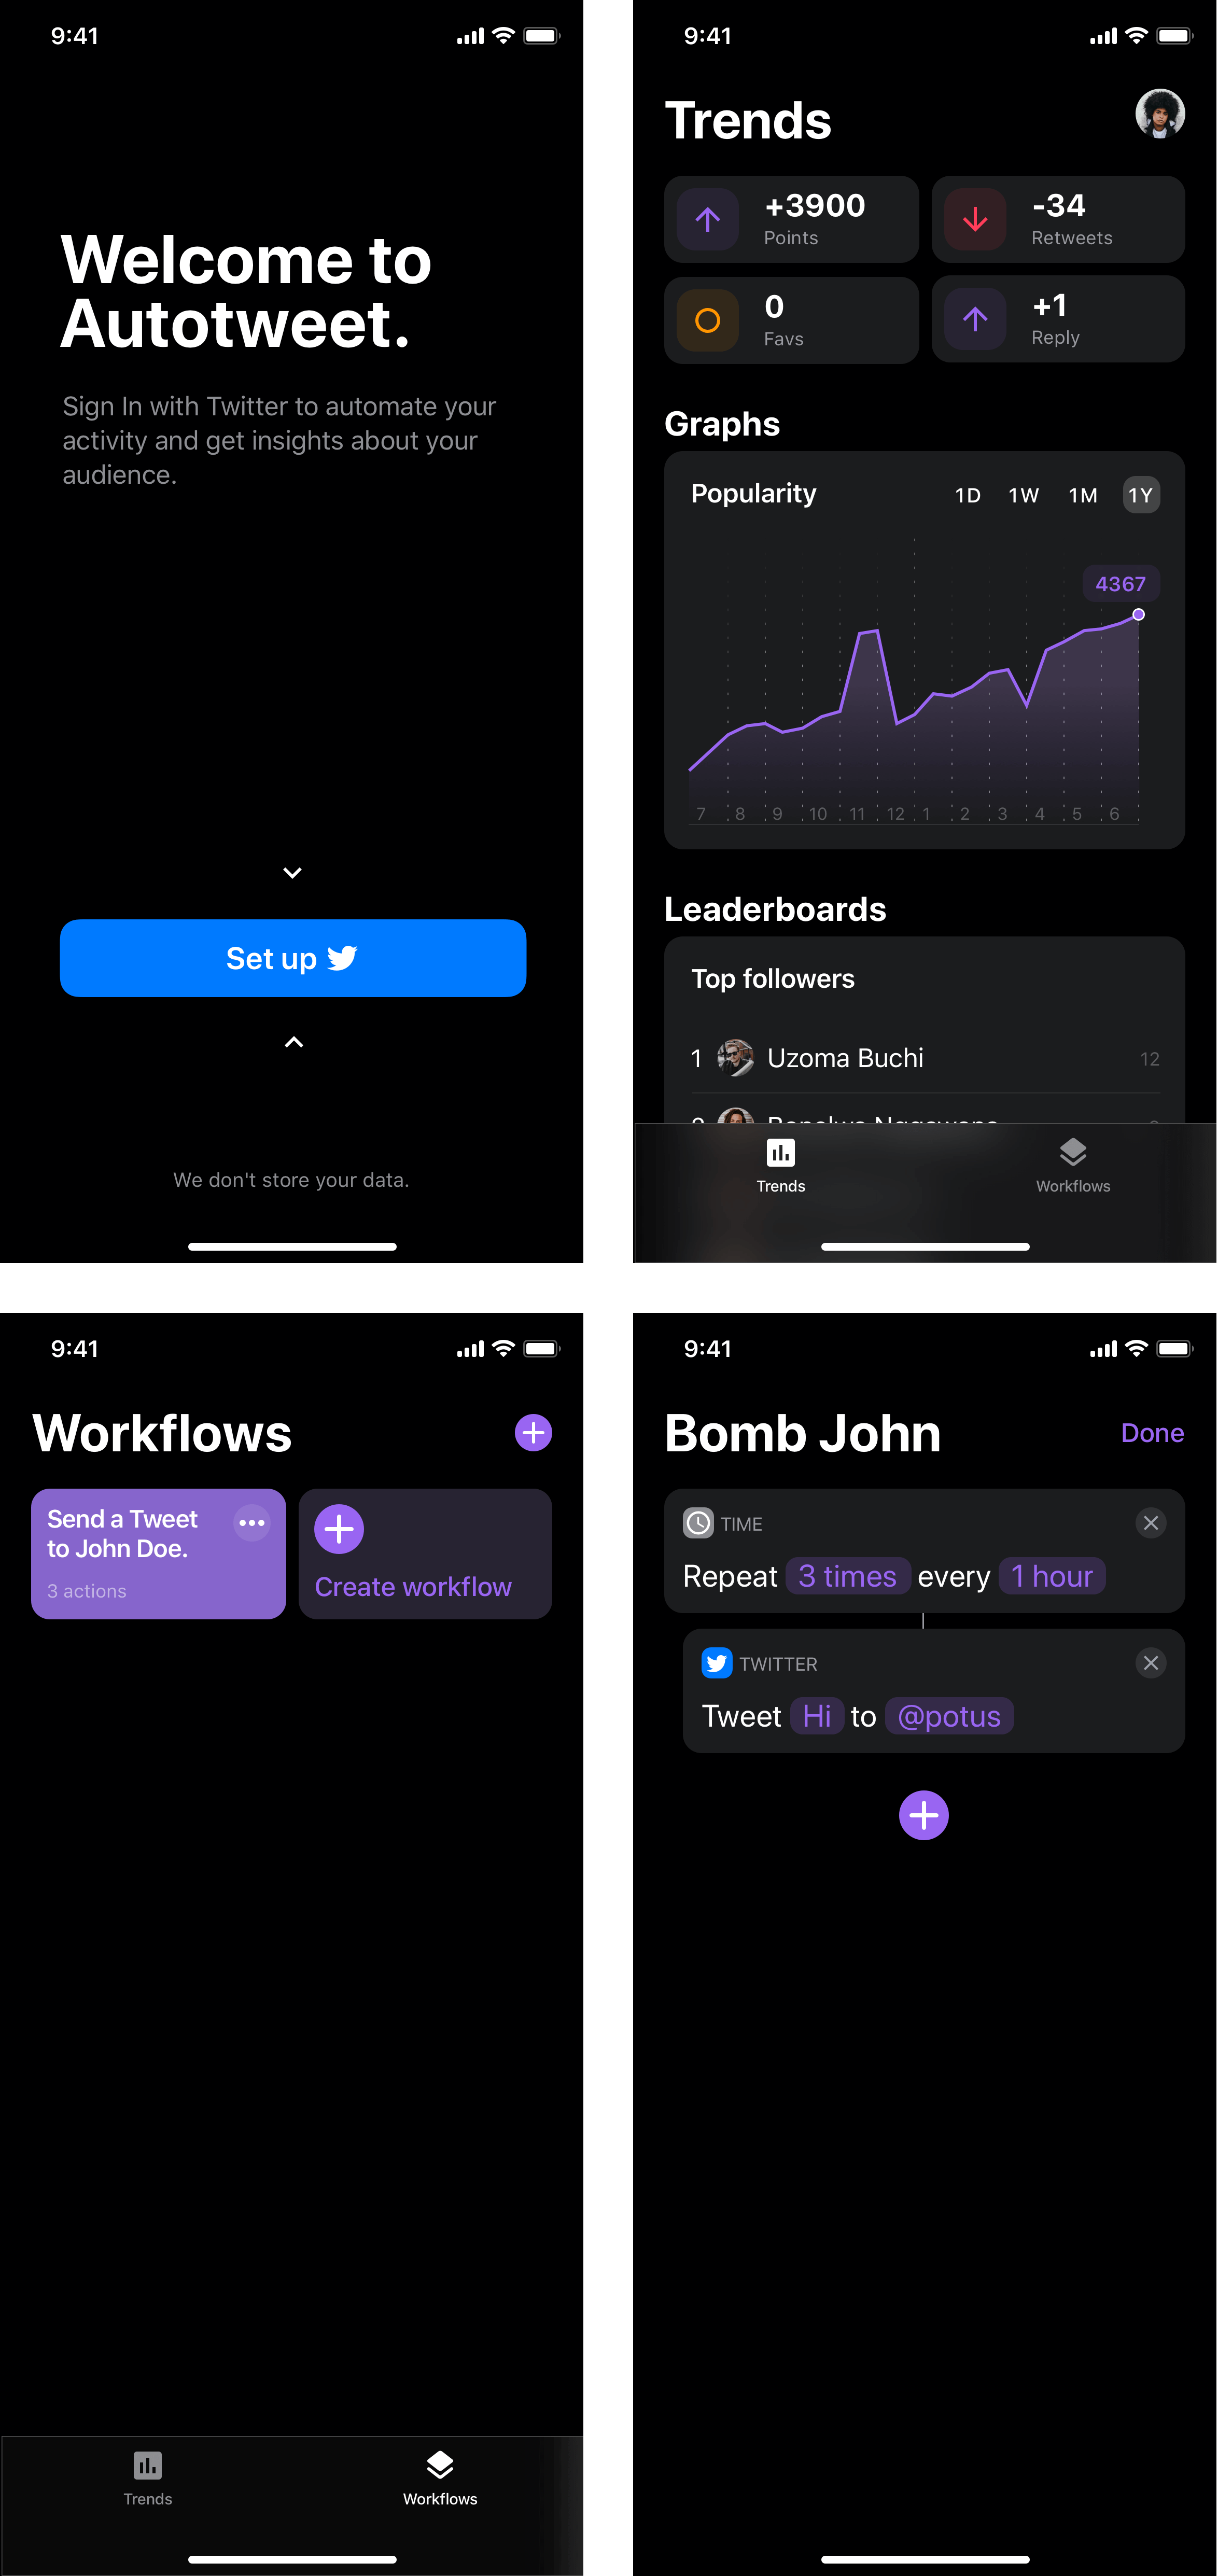
\includegraphics[width=8cm]{gui}
    \caption{Login, Trend view and Workflows view}
    \label{fig:gui}
\end{figure}

\begin{figure}[htp]
    \centering
    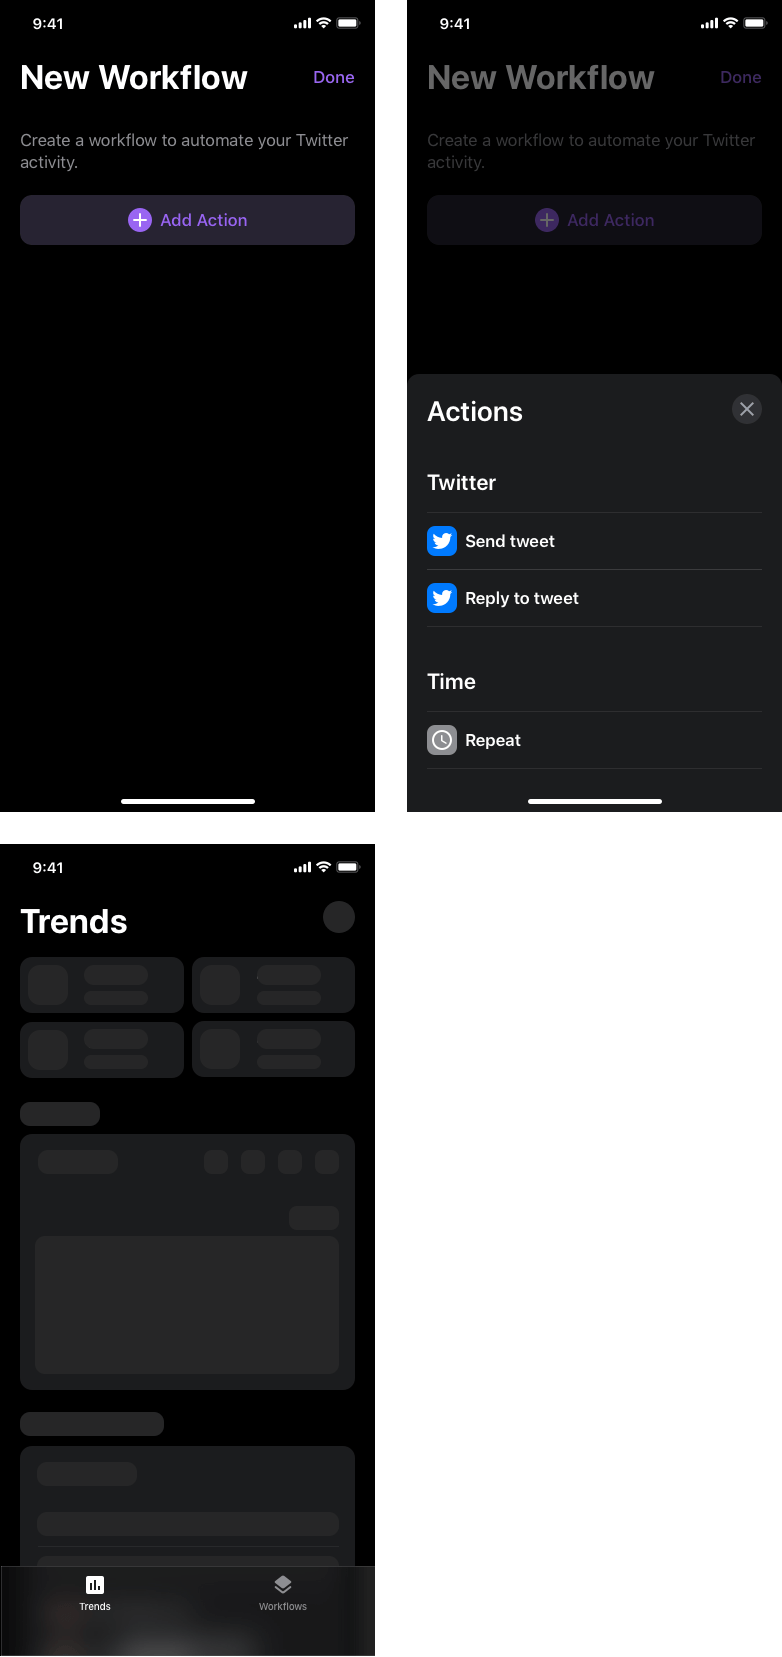
\includegraphics[width=8cm]{gui2}
    \caption{Initial State, Action menu and skeletons}
    \label{fig:gui2}
\end{figure}

\chapter{Development}

\section{Technologies}
We had initially planned to carry out the project entirely in React Native. When we wanted to link our application to the Twitter API, we encountered problems with the CORS model. The Twitter API does not support CORS. Thus, it was impossible to send requests to it from a controlled environment such as the browser. To overcome this problem, we tried several solutions. First, we built a reverse-proxy between the API and our client to transmit the requests. We experimented using Node, Golang, Deno and Nginx. While making these proxies, it turned out that there were a lot of edge-cases where the connection didn't work. We gave up on the idea of building it ourselves. We then turned our attention to a third party solution called 'cors-anywhere'. It worked.
However, the lack of a JS Twitter library quickly slowed us down. We therefore looked for other platforms that could replace Javascript. Go caught our attention with the `go-twitter' library. From that moment on, we started to gradually build a Go server between the client and Twitter.

\section{Architecture}
As we have no domain expertise on the Twitter API, we let the client's structure grow organically rather than planning it meticulously in advance. We decided to isolate the responsibilities as soon as possible and organized the components by domain. Very early on, we ran into problems with state management. Some states, notably those of authentication, needed to be shared across the entire application. We tried to do this with "Context", but it wasn't enough. We finally decided to use a Flux architecture with the Redux library. 
Redux applications are usually heavy in boilerplate. We made sure that this is not the case with our client by using an additional library called "redux-toolkit". There is no notion of container or connected component. A component uses the redux store if it needs it. 
We also have isolated the API request logic into a specific folder named `api`. It takes the form of an API client library.

\section{Go server}

We approached the architecture of the server in the same way as with the client. It started out as a simple proxy server but it evolved to a full-blown API. Its architecture is simple and respects Go's philosophy. In the beginning, there was only one file consisting of a proxy in front of the Twitter Oauth system. It evolved into multiple packages such as Trends, Metrics and Automation.
In order to document the server's REST API to the consumers, an OpenAPI specification is maintened in parralel with this server. Our server is stateless so access tokens are encoded from the client to the server using HTTP basic auth in each request.

The server is tightly coupled to the mobile app's features and conforms to a Backend For Frontend pattern.

\section{Tests}
We did not find the need to test on the client because there was no regression and the API query logic is simple. However, we tested custom encoding functions on the server that had to be reliable. These tests no longer exist today because we have concluded that the best way to make the code reliable is to use field-tested third party libraries rather than reinventing the wheel.

\begin{figure}[htp]
    \centering
    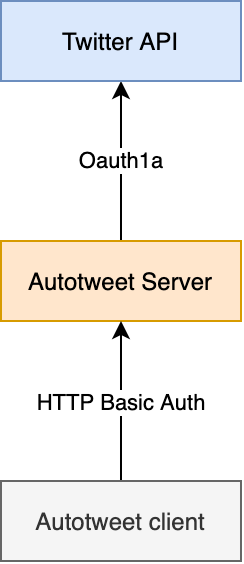
\includegraphics[width=3cm]{diagram1}
    \caption{Authentication flow}
    \label{fig:diagram1}
\end{figure}

\chapter{Difficulties}

\section{Graph Widget}

We wanted the graph widget to be exactly the same as the one we designed in the mockup. This means that the graphics library had to support gradients, dotting and axis customization. We experimented with React Native charting libraries but we couldn't achieve the desired result. As the most customizable JS charting libraries are made for the DOM, we needed them to replicate the mockup. Our solution was to render the chart server-side and pass the HTML in a Webview component. The result is almost perfect. The only drawback is the loading time, which is slightly long.

\section{Loading times}

Requests from the app sometimes spawn multiple requests on the server against the Twitter API to achieve the desired results. This slows down the user experience and can make it frustrating. To make up for that, we made skeleton screens out of every connected component to distract the user when data is loading as illustrated in figure \ref{fig:skeleton-loading}.

\begin{figure}[htp]
    \centering
    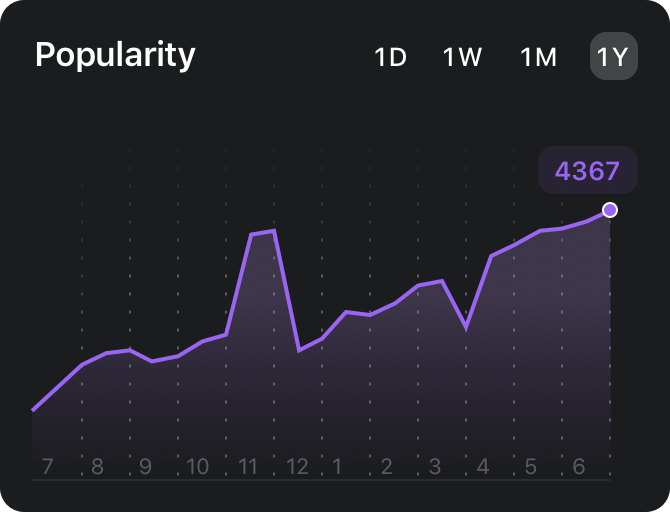
\includegraphics[width=5cm]{graph-widget}
    \caption{The graph widget}
    \label{fig:graph-widget}
\end{figure}

\begin{figure}[htp]
    \centering
    
\includegraphics[width=4cm]{skeleton-loading}
    \caption{Loading state}
    \label{fig:skeleton-loading}
\end{figure}


\begin{figure}[htp]
    \centering
    
\includegraphics[width=4cm]{skeleton-success}
    \caption{Success state}
    \label{fig:skeleton-success}
\end{figure}
\end{document}
